\chapter{Aspectos Generales}
\section{Aspectos Generales}
\subsection{Descripción del Problema}
Uno de los sentidos más importantes de los seres humanos es la visión. Ésta es empleada para obtener la información visual del entorno físico. Según Aristóteles, “Visión es saber que hay y donde mediante la vista”. De hecho, se calcula que más del 75\% de las tareas del cerebro son empleadas en el análisis de la información visual. El refrán popular de “Una imagen vale más que mil palabras” tiene mucho que ver con los aspectos cognitivos de la especie humana. Casi todas las disciplinas científicas emplean utillajes gráficos para transmitir conocimiento\footnote[1]{Visión Humana, fuente: Sistemas Adaptativos y Bioinspirados en Inteligencia Artificial\href{http://sabia.tic.udc.es/}{(S.A.B.I.A.)}}.

Uno de los más grandes concursos a nivel mundial en clasificación de imágenes reporta que las técnicas tradicionales (como las técnicas de extracción de características en imágenes estáticas: \textit{Principal component analysis} (PCA), \textit{Edges detector}, \textit{Gabor waveled}; Video: PCA, \textit{Discrete cosine transform} (DCT), \textit{optical flow} e \textit{image difference}) están siendo superadas por técnicas de \textit{Deep Learning} basadas en el proceso cerebral humano. Dicho éxito se debe a que las técnicas tradiciones requieren de un ambiente controlado y no son tolerables a cambios como: traslación, rotación y escalado, por otro lado las técnicas de \textit{Deep Learning} demustran ser mas robustas y efectivas frente a estos tipos de cambios\footnote[2]{\textit{Deep Learning} vs. \textit{Machine Learning} fuente: \href{http://www.image-net.org/}{Analytics Vidhya}}.
	
Diversas actividades cotidianas necesitan del reconocimiento de imágenes, tal es el caso del reconocimiento de expresiones faciales, que en los últimos años se ha convertido en una de las tareas más estudiadas por investigadores en todo el mundo, con el fin de alcanzar un margen de error minimo para posteriormente centrarse en el desarrollo de aplicaciones en distintos campos, como: estudio de marketing, interacción hombre-máquina, psicología y análisis educativo \footnote[3]{Las expresiones faciales de las emociones, historia y aplicaciones, fuente: \href{http://medina-psicologia.ugr.es/cienciacognitiva/?p=664}{Ciencia Cognitiva}}, las cuales han sido abordada por diferentes técnicas tradicionales no obteniendo los resultados prometedores en imagenes reales que contienen distintos tipos de variaciones (mencionados en el parrafo anterior) limitando asi la implementacion y desarrollo de aplicaciones utiles para el bien comun (aplicaciones antes mencionadas).

\subsection{Identificación del Problema}
Las técnicas tradicionales para el reconocimiento de expresiones faciales usadas en la actualidad necesitan de un ambiente controlado (iluminacion constante, alta calidad de imagen, poco ruido, imagen sin oclusión), y no son tolerables a cambios como rotación, traslación, escalado, limitando asi la creacion de aplicaciones con imagenes del mundo real(imagenes obtenidas a partir de camaras de seguridad) . Por lo que hay la necesidad de usar nuevas técnicas del estado del arte que nos permitiran obtener mejores resultados superando asi la limitacion antes mencionada.

\section{Antecedentes}
Se muestra una lista de trabajos resaltantes que hacen uso de tecnicas de \textit{Deep Learning}, los cuales sirvieron de inspiración y fuente de información valiosa en el desarrollo de este trabajo. Tambien se presentan trabajos dedicados al reconocimiento de expresiones faciales utilizando técnicas tradicionales de vision por computador y \textit{Machine Learning}.


\vspace{1cm}
\textbf{Métodos de Reconocimiento de expresiones faciales con ténicas tradicionales y \textit{Machine learning}.} 
Muchos abordages fueron propuestos para la tarea de reconocimiento de expresiones faciales. Zhong et. al   \cite{zhong2012learning} propone un método para el reconocimiento de expresiones faciales basado en \textit{patches} informativos de expresiones faciales (eg. ojos, mejillas, boca, etc ) de los rostros humanos contenidos en las imagenes. Asi, introduce un marco de aprendizaje por tareas multiples (MTSL) de dos etapas para ubicar de manera eficiente los \textit{patches} discriminativos en las imagenes con contenido facial. La primera etapa consiste en extraer un conjunto de \textit{patches} por cada expresion facial dentro de un conjunto de datos de entrenamiento. En la segunda parte del MTSL, extraido el conjunto  de patches por cada expresion facial en el conjunto de datos de entrenamiento dos tareas son desarrollados, el reconocimiento de expresion facial y verificacion facial.  Estas dos tareas son integrados para aprender de los patches obtenidos con anterioridad. El aprendizaje tiene como objetivo determinar cuales son los especificos \textit{patches} faciales que corresponden a cada expresion facial. Finalmente, un clasificador SVM es entrenado para reconocer las caracteristicas contenidas en los patches para una de las seis expresiones faciales consideradas en este trabajo. Por otro lado, Almaev et al \cite{almaev2013local} propone un descriptor dinámico de apariencias \textit{Local Gabor Binary Patterns de Three Ortogonal Planes}(LGBP-TOP) donde, analizando la textura espacial y dinamica, y combinado con filtros de gabor logra un alto nivel de precision en el reconocimiento de expresiones faciales en tiempo real. Ademas, el descriptor propuesto es robusto a errores en la alineacion rotacional propios de la captura de registros.
Ghayoumi et. al \cite{ghayoumi2014integrated} propone la integracion de dos métodos para el reconocimiento de expresiones faciales. \textit{Locality Sensitive Hashing} (LSH), \textit{Principal Component Analysis} (PCA) y \textit{Linear Discriminant Analysis} (LDA)  son los tres métodos utilizados para el reconocimiento de expresiones faciales en este trabajo.
Para reconocer una expresion facial son extraidos los vectores de caracteristicas de dos regiones mas informativas del rostro, la región de los ojos y la región de la boca. El LSH esta compuesto por funciones hash los cuales son usados para mapear los vectores de caracteristicas extraidos de las imagenes en un bloque de colisiones, donde cada bloque esta registrado como la locacion de vectores de caracteristicas pertenecientes a una especifica expresion facial apriori. Asi, se logra reducir redundancia en el espacio de representación de las imagenes respecto a las imagenes que pertencen a la mismo tipo de expresion facial. Luego de este paso son aplicados los metodos de reducción de dimensionalidad PCA y LDA  para aliviar la complejidad computacional, ademas de reducir redundancia en los datos. Por ultimo, es entrenado un clasificador SVM con los datos obtenidos despues de aplicado los métodos de reducción de dimensionalidad.



\textbf{Técnicas de \textit{Deep Learning}.} Muchos de los avances en visión por computador, procesamiento del lenguaje natural, bioinformatica y otros campos de investigación se debe a la utilización de métodos y técnicas de inteligencia artificial, especificamente técnicas de \textit{machine lerning} y \textit{Deep Learning}. Este último, es el causante de una gran impacto en el avance técnologico con relacionamiento directo en el mundo comercial (carros autónomos, chatboots, creación de nuevos farmacos por computador, etc).  Yan Lecunn  et. al \cite{2lecun1998gradient} introduce uno de los primeros trabajos con redes neuronales convolucionales, un tipo especial del deep learning. En este trabajo, muestra la potencialidad de la técnica de aprendizaje basado en gradiente. Esta técnica es utilizado en el entrenamiento de una Multilayer perceptron via el algoritmo de backpropagation. Es diseñado una Red Neuronal Convolucional para tratar con la variabilidad de forma 2D en imagenes para el reconocimiento de digitos escritos a mano. tambien es introducido dos sistemas on-line para el reconocimiento de documentos escritos a mano. Para controlar los componentes del sistema tales como la extracción, segmentación, reconocimiento y modelage del lenguaje; es introducido un nuevo paradigma de aprendizaje llamado \textit{Graph Transformer networks}. Ademas, es descrito la pontencialidad del \textit{Graph transformer networks} aplicado a la lectura de cheques de banco. Donde, las Redes Neuronales Convolucionales para el reconocimiento de caracteres combinado con técnicas de entrenamiento global proporcionaron un alto rendimiento.Esto fue demostrado en el area comercial al ser capaz el modelo introducido de leer cheques personales de forma automatizada, logrando leer millones de cheques por dia. Mas tarde, Krizhevsky et. al \cite{8krizhevsky2012imagenet} propone una arquitectura de Red Neuronal Convolucional profunda que es entrenado para clasificar 1.2 millones de imagenes en alta resolucion en 1000 categorias. La red propuesta en este trabajo llega a estar compuesto por 60 millones de parametros y 650000 neuronas. Para el entrenamiento fue usaada GPUs para acelerar el computo de multiplicaciones matriciales requeridas en la operacion de convolucion. Ademas, el entrenamiento duro 2 semanas.
Este trabajo logra el estado del arte en clasificacion de imagenes a gran escala en la competicion ILSVRC-2012.
Este trabajo, logro reducir el error de clasificación de imagenes en la base de datos ImageNet de 26.2\% a 15.3 \%. Siendo asi, uno de los trabajos con mas impacto en visión por computador. Asi, vemos que una de las principales desventajas de los métodos basados en extracción de caracteristicas diseñadas a mano es el tiempo de computo lo que les dificulta ser escalables, requisito principal para aplicaciones en el mundo real.
ademas, estos métodos solo cubren una parte especifica de casos, esto debido a las asunciones que se toman para casos especificos que no logran cubrir lo necesario para crear modelos generalizables. Por otro lado, los métodos de Deep Learning logran crear modelos generalizables y escalables. Asi, esto nos motivo para desarrollar una arquitectura de red neuronal convolucional para el reconocimiento de expresiones faciales.



\section{Objetivos}
\subsection{Objetivo General}
Desarrollar una arquitectura de Red Neuronal Convolucional que sea capaz de obtener niveles de precision confiables (con un minimo margen de error) en el reconocimiento de expresiones faciales, permitiendo asi contribuir en el desarrollo de futuras aplicaciones del mundo real que sirvan para el beneficio de la sociedad.
\subsection{Objetivos Específicos}
\begin{itemize}
\item Selección de las bases de datos de expresiones faciales y transformación de datos a un formato estandar para su posterior utilizacion.
\item Investigar los filtros de convolucion para la correcta seleccion de los parametros.
\item Investigar la funcion de submuestreo para la correcta selección de los parametros. 
\item Investigar las funciones de activación y funciones de normalizacion para la correcta selección de los parametros.
\item Diseñar la arquitectura propuesta(configuracion de parametros, numero de capas y funciones de activacion y normalizacion), basandonos en los objetivos previos.
\item Entrenar la arquitectura propuesta.	
\item Evaluar el modelo creado a partir de la arquitectura propuesta.
\item Analizar e interpretar los resultados
\end{itemize}

\section{Alcances}
En este trabajo de investigacion se lograron los siguientes alcances.

\begin{itemize}
\item Se propuso una nueva arquitectura para el reconocimiento de expresiones faciales, basada en las Redes Neuronal Convolucional, capaz de obtener altos niveles de precision que seran de utilidad para el desarrollo de futuras aplicaciones del mundo real.
\item Se creo una nueva base de datos, la cual fue resultado de la union de las dos bases de datos antes mencionadas(FER2013 y CK+).
\item Contribuimos con la comunidad academica del país y la region brindandoles informacion de un tema de investigación actual que servira como base para el desarrollo de futuras aplicaciones y trabajos relacionados.
\end{itemize}
 

\section{Justificación}
En la actualidad se ha dado más realce a algunas disciplinas de la inteligencia artificial como: \textit{Machine Learning} y \textit{Deep Learning}, disciplinas que brindan distintas técnicas que están dando solución a problemas de clasificación de imágenes, comprensión de escena, análisis de sentimientos y otros. Así es el caso de la visión artificial donde las Redes Neuronales Convolucionales está proporcionando mejores resultados en comparación con algoritmos y técnicas tradicionales.

En este trabajo, presentamos un estudio resumido de la investigación hecha en \textit{Deep Learning} que servirá tanto para los investigadores como para los lectores. También este trabajo ayudara para el desarrollo de futuros proyectos de clasificación de imágenes en distintos campos (seguridad, medicina y biología, internet y la nube, entretenimiento, maquinas autónomas y otros)\footnote[4]{Aplicaciones de Deep Learning, fuente: \href{https://developer.nvidia.com/deep-learning}{NVIDIA} GPUs - el motor del aprendizaje profundo(deep learning)}.


\section{Metodología}
Dada la naturaleza del trabajo de investigación, se utilizó los métodos de investigación bibliográfica, explorativa y aplicativa. Bibliográfica ya que se recogió y analizo información para obtener conocimientos previos sobre \textit{Deep Learning} y el detector \textit{Haar Cascade}. Explorativa porque se seleccionó información relevante procedente de la etapa de investigación bibliográfica, para la construcción de la arquitectura de una Red Neuronal Convolucional basándonos en trabajos previos relacionados con la línea de investigación. Aplicativa por que se utilizaron los conocimientos adquiridos \cite{19sabino1994hacer}\cite{23silva2001metodologia}.


\section{Limitaciones}
\begin{itemize}
\item Dificil acceso a herramientas tecnológicas de hardware, principalmente GPU's de alta capacidad, necesarias para la fase de entrenamiento de la Red Neuronal Convolucional. Por consiguiente, la solución es alquilar servidores en la nube especializados en el entrenamiento de arquitecturas de \textit{Deep Learning}.
\item Carencia de organizaciones peruanas que brinden bases de datos para poder utilizarlos en la fase de entrenamiento ya que se requiere miles de imágenes (imágenes de acuerdo al proyecto de investigación en el que se trabaje, como: rostros, danzas, señas, sitios arqueológicos y entre otros) para que se cree un modelo eficiente y robusto, llevando a utilizar base de datos de organizaciones extranjeras que fomentan la investigación en esta área.
\end{itemize}
\newpage
\section{Cronograma de Actividades}
\begin{table}[!htb]
    \centering
    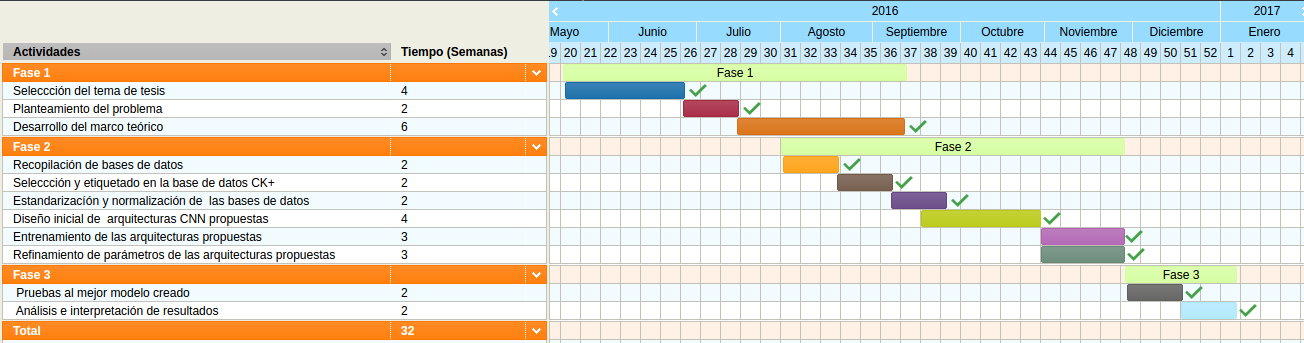
\includegraphics[angle=90,width=60mm]{Imagenes/cronograma.png}
    \caption{Cronograma de actividades}
    \label{tab:tab1}
\end{table}


